\chapter{Proofs of background facts}
\lbl{app:proofs}


This appendix consists of proofs deferred from the main text.  


\section{Forms of the chain rule for entropy}
\lbl{sec:chain}
\index{chain rule!forms of}


In Remark~\ref{rmk:ent-chain-simp}, it was asserted that although the
chain rule
\[
H\bigl( \vc{w} \of (\p^1, \ldots, \p^n)\bigr)
=
H(\vc{w}) + \sum_{i = 1}^n w_i H(\p^i)
\]
for Shannon entropy appears to be more general (that is, stronger) than the
versions used by some previous authors, straightforward inductive arguments
show that it is equivalent to those special cases.
Remark~\ref{rmk:q-ent-char-hist} made a similar assertion for the
$q$-logarithmic entropies $S_q$, where the equation becomes
\[
S_q\bigl( \vc{w} \of (\p^1, \ldots, \p^n)\bigr)
=
S_q(\vc{w}) + \sum_{i \in \supp(\vc{w})} w_i^q S_q(\p^i).
\]
Here we prove those claims.

In Lemma~\ref{lemma:ch-forms} below, part~\bref{part:cf-full} is the
general form of the chain rule, parts~\bref{part:cf-l}
and~\bref{part:cf-twotop} are the special cases used by other authors, and
part~\bref{part:cf-int} is an intermediate case that is helpful for the
proof.  Each of the four parts corresponds to a certain type of composition
of probability distributions, depicted as a tree in
Figure~\ref{fig:comp-trees}.  

Rather than working with sums over the support of $\vc{w}$, in this lemma
we adopt the convention that $0^q = 0$ for all $q \in \R$.

\begin{lemma}
\lbl{lemma:ch-forms}
Let $q \in \R$.  Let $( I \from \Delta_n \to \R)_{n \geq 1}$ be a sequence
of symmetric functions.  The following are equivalent:
% 
\begin{enumerate}
\item 
\lbl{part:cf-full}
for all $n, k_1, \ldots, k_n \geq 1$, $\vc{w} \in \Delta_n$, and $\p^i \in
\Delta_{k_i}$, 
\[
I\bigl( \vc{w} \of (\p^1, \ldots, \p^n)\bigr) 
= 
I(\vc{w}) +
\sum_{i = 1}^n w_i^q I(\p^i);
\]

\item
\lbl{part:cf-l}
for all $n \geq 1$, $\vc{w} \in \Delta_n$, and $p \in [0, 1]$,
\[
I\bigl(w_1 p, w_1(1 - p), w_2, \ldots, w_n)
=
I(\vc{w}) + w_1^q I(p, 1 - p);
\]

\item
\lbl{part:cf-int}
for all $n, k \geq 1$, $\vc{w} \in \Delta_n$, and $\vc{p} \in \Delta_k$,
\[
I(w_1 p_1, \ldots, w_1 p_k, w_2, \ldots, w_n)
=
I(\vc{w}) + w_1^q I(\vc{p});
\]

\item
\lbl{part:cf-twotop}
for all $k, \ell \geq 1$, $\p \in \Delta_k$, $\vc{r} \in \Delta_\ell$, and
$w \in [0, 1]$, 
% 
\begin{multline*}
I(wp_1, \ldots, wp_k, (1 - w)r_1, \ldots, (1 - w)r_\ell)        \\
=
I(w, 1 - w) + w^q I(\p) + (1 - w)^q I(\vc{r}).
\end{multline*}
\end{enumerate}
\end{lemma}
% 
Much of the following argument goes back to Feinstein
(\cite{Fein}, p.~5--6).%
%
\index{Feinstein, Amiel}

\begin{figure}
\lengths
\begin{picture}(60,44)(30,-1)
\cell{60}{23}{c}{\includegraphics[height=40\unitlength]{composite2}}
\cell{60}{25}{c}{$\cdots\cdots$}
\cell{60}{10}{c}{$\cdots$}
\cell{41}{5}{c}{$\cdots$}
\cell{79}{5}{c}{$\cdots$}
% 
\cell{42}{28}{c}{$w_1$}
\cell{78}{28}{c}{$w_n$}
\cell{33}{9}{c}{$p^1_1$}
\cell{51}{9}{c}{$p^1_{k_1}$}
\cell{71}{9}{c}{$p^n_1$}
\cell{88}{9}{c}{$p^n_{k_n}$}
% 
\cell{30}{23}{l}{\bref{part:cf-full}}
% \put(60,43){\line(0,-1){90}}
\end{picture}%
\begin{picture}(60,44)(22,-1)
\cell{57.5}{23}{c}{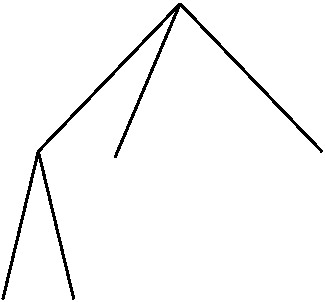
\includegraphics[height=40\unitlength]{compositeL}}
\cell{65}{25}{c}{$\cdots\cdots$}
% 
\cell{42}{28}{c}{$w_1$}
\cell{51}{28}{c}{$w_2$}
\cell{78}{28}{c}{$w_n$}
\cell{36}{9}{r}{$p$}
\cell{46}{9}{l}{$1 - p$}
% 
\cell{30}{23}{l}{\bref{part:cf-l}}
% \put(60,43){\line(0,-1){90}}
\end{picture}
\begin{picture}(60,40)(30,3)
\cell{56.2}{23}{c}{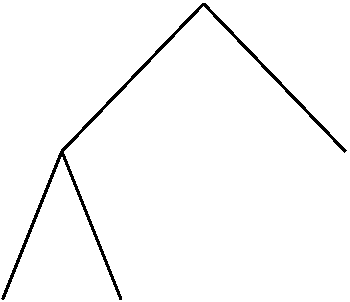
\includegraphics[height=40\unitlength]{compositeintermediate}}
\cell{60}{25}{c}{$\cdots\cdots$}
\cell{41}{5}{c}{$\cdots$}
% 
\cell{42}{28}{c}{$w_1$}
\cell{78}{28}{c}{$w_n$}
\cell{33}{9}{c}{$p_1$}
\cell{51}{9}{c}{$p_k$}
% 
\cell{30}{23}{l}{\bref{part:cf-int}}
\end{picture}%
\begin{picture}(60,40)(22,3)
\cell{60}{23}{c}{\includegraphics[height=40\unitlength]{compositetwotop}}
\cell{48}{5}{c}{$\cdots$}
\cell{72}{5}{c}{$\cdots$}
% 
\cell{50}{28}{r}{$w$}
\cell{70}{28}{l}{$1 - w$}
\cell{41}{9}{c}{$p_1$}
\cell{57.5}{9}{c}{$p_k$}
\cell{63.5}{9}{c}{$r_1$}
\cell{79.5}{9}{c}{$r_\ell$}
% 
\cell{30}{23}{l}{\bref{part:cf-twotop}}
\end{picture}%
\caption{Shapes of composites used in the four parts of
  Lemma~\ref{lemma:ch-forms}.}
\lbl{fig:comp-trees}
\end{figure}

\begin{proof}
% We prove that
% \bref{part:cf-full}$\textimplies$\bref{part:cf-l}$\textimplies$\bref{part:cf-int}$\textimplies$\bref{part:cf-twotop}$\textimplies$\bref{part:cf-full}. 
% 
% Taking $k_1 = 2$ and $k_2 = \cdots = k_n = 1$ in

Trivially, \bref{part:cf-full} implies~\bref{part:cf-l}.

Assuming~\bref{part:cf-l}, we prove~\bref{part:cf-int} by induction on
$k$.  The case $k = 1$ reduces to the statement that $I(\vc{u}_1) = 0$,
which follows by taking $n = 1$ in~\bref{part:cf-l}.  Now let $k \geq 2$,
and assume the result for $k - 1$.

Let $n \geq 1$, $\vc{w} \in \Delta_n$, and $\vc{p} \in \Delta_k$.  By
symmetry, we can assume that $p_k < 1$.  Using the inductive hypothesis, we
have
% 
\begin{align*}
&
I(w_1 p_1, \ldots, w_1 p_k, w_2, \ldots, w_n)   \\
&
=
I\biggl( 
w_1(1 - p_k) \cdot \frac{p_1}{1 - p_k}, \ldots,
w_1(1 - p_k) \cdot \frac{p_{k - 1}}{1 - p_k}, 
w_1 p_k, w_2, \ldots, w_n
\biggr) \\
&
=
I\bigl( w_1(1 - p_k), w_1 p_k, w_2, \ldots, w_n\bigr)
+
\bigl( w_1 (1 - p_k) \bigr)^q
I\biggl( \frac{p_1}{1 - p_k}, \ldots, \frac{p_{k - 1}}{1 - p_k} \biggr),
\end{align*}
% 
which by~\bref{part:cf-l} is equal to
\[
I(\vc{w}) 
+ 
w_1^q \biggl\{
I(1 - p_k, p_k) 
+
(1 - p_k)^q
I\biggl( \frac{p_1}{1 - p_k}, \ldots, \frac{p_{k - 1}}{1 - p_k} \biggr)
\biggr\}.
\]
But by the inductive hypothesis again, the term $\{\cdots\}$ is equal to
\[
I\biggl(
(1 - p_k) \cdot \frac{p_1}{1 - p_k}, \ldots, 
(1 - p_k) \cdot \frac{p_{k - 1}}{1 - p_k},
p_k
\biggr)
=
I(\p),
\]
completing the induction.

Now assuming~\bref{part:cf-int}, we prove~\bref{part:cf-twotop}.  Let $k,
\ell \geq 1$, $\p \in \Delta_k$, $\vc{r} \in \Delta_\ell$, and $w \in [0,
  1]$.  Using~\bref{part:cf-int}, we have
% 
\begin{multline*}
I(wp_1, \ldots, wp_k, (1 - w)r_1, \ldots, (1 - w)r_\ell)        \\
=
I\bigl(w, (1 - w)r_1, \ldots, (1 - w)r_\ell\bigr)
+
w^q I(\p).
\end{multline*}
% 
By symmetry and~\bref{part:cf-int} again, this in turn is equal to 
\[
I(w, 1 - w) + (1 - w)^q I(\vc{r}) + w^q I(\vc{p}),
\]
proving~\bref{part:cf-twotop}.

Finally, assume~\bref{part:cf-twotop}. We prove~\bref{part:cf-full} by
induction on $n$.  The case $n = 1$ just states that $I(\vc{u}_1) = 0$,
which follows from~\bref{part:cf-twotop} by taking $k = \ell = 1$.  Now let
$n \geq 2$, and assume the result for $n - 1$.

Let $k_1, \ldots, k_n \geq 1$, $\vc{w} \in \Delta_n$, and $\p^i \in
\Delta_{k_i}$.  By symmetry, we can assume that $w_1 > 0$.  Write
\[
\vc{p}^{12} 
=
\biggl( 
\frac{w_1}{w_1 + w_2} p^1_1, \ldots, \frac{w_1}{w_1 + w_2} p^1_{k_1},
\frac{w_2}{w_1 + w_2} p^2_1, \ldots, \frac{w_2}{w_1 + w_2} p^2_{k_2}
\biggr)
\in 
\Delta_{k_1 + k_2}.
\]
Then
\[
\vc{w} \of (\p^1, \ldots, \p^n)
=
(w_1 + w_2, w_3, \ldots, w_n) \of (\p^{12}, \p^3, \ldots, \p^n),
\]
so by inductive hypothesis,
% 
\begin{multline}
\lbl{eq:41-mid}
I\bigl( \vc{w} \of (\p^1, \ldots, \p^n) \bigr) \\
=
I(w_1 + w_2, w_3, \ldots, w_n) + (w_1 + w_2)^q I(\p^{12}) 
+ \sum_{i = 3}^n w_i^q I(\p^i).
\end{multline}
% 
On the other hand, by~\bref{part:cf-twotop},
\[
I(\p^{12})
=
I\biggl( \frac{w_1}{w_1 + w_2}, \frac{w_2}{w_1 + w_2} \biggr)
+
\biggl( \frac{w_1}{w_1 + w_2} \biggr)^q I(\p^1)
+
\biggl( \frac{w_2}{w_1 + w_2} \biggr)^q I(\p^2).
\]
Substituting this into~\eqref{eq:41-mid}, we deduce that $I\bigl( \vc{w}
\of (\p^1, \ldots, \p^n) \bigr)$ is equal to
% 
\begin{equation}
\lbl{eq:cf-last}
I(w_1 + w_2, w_3, \ldots, w_n) 
+ 
(w_1 + w_2)^q I\biggl( \frac{w_1}{w_1 + w_2}, \frac{w_2}{w_1 + w_2} \biggr)
+
\sum_{i = 1}^n w_i^q I(\p^i).
\end{equation}
% 
But applying the inductive hypothesis to the composite
\[
\vc{w}
=
(w_1 + w_2, w_3, \ldots, w_n)
\of
\biggl( \biggl(  \frac{w_1}{w_1 + w_2}, \frac{w_2}{w_1 + w_2} \biggr),
\vc{u}_1, \ldots, \vc{u}_1 \biggr)
\]
gives
\[
I(\vc{w})
=
I(w_1 + w_2, w_3, \ldots, w_n)
+ 
(w_1 + w_2)^q I\biggl( \frac{w_1}{w_1 + w_2}, \frac{w_2}{w_1 + w_2} \biggr)
\]
(recalling that $I(\vc{u}_1) = 0$).  Hence the
expression~\eqref{eq:cf-last} reduces to
\[
I(\vc{w}) + \sum_{i = 1}^n w_i^q I(\p^i),
\]
proving~\bref{part:cf-full}.
\end{proof}


\section{The expected number of species in a random sample}
\lbl{sec:hsg}
\index{expected number of species in sample}
\index{Hurlbert, Stuart!Smith--Grassle@--Smith--Grassle index}


Here we prove the result stated in Example~\ref{eg:hsg}, which expresses the
diversity index of Hurlbert, Smith and Grassle in terms of the Hill numbers
$D_q(\p)$.

Recall that we are modelling an ecological community with $n$ species via
its relative abundance distribution, and that $\hsg_m(\p)$ denotes the
expected number of different species represented in a random sample with
replacement of $m$ individuals.  The claim is that
\[
\hsg_m(\p)
=
\sum_{q = 1}^m (-1)^{q - 1} \binom{m}{q} D_q(\p)^{1 - q}.
\]

Define random variables $X_1, \ldots, X_n$ by
\[
X_i     
=
\begin{cases}
1       &\text{if species } i \text{ is present in the sample}, \\
0       &\text{otherwise}.
\end{cases}
\]
Then $\sum_{i = 1}^n X_i$ is the number of different species in the sample,
so
% 
\begin{align*}
\hsg_m(\p)      &
=
\Ex\Biggl( \sum_{i = 1}^n X_i \Biggr)  
=
\sum_{i = 1}^n \Ex(X_i) \\
&
=
\sum_{i = 1}^n \Pr(\text{species } i \text{ is present in the sample})  \\
&
=
\sum_{i = 1}^n \bigl( 1 - (1 - p_i)^m \bigr),
\end{align*}
% 
as Hurlbert%
%
\index{Hurlbert, Stuart} 
% 
observed (equation~(14) of~\cite{Hurl}).  It follows that
% 
\begin{align*}
\hsg_m(\p)      &
=
n - \sum_{i = 1}^n \sum_{q = 0}^m \binom{m}{q} (-p_i)^q \\
&
=
n - \sum_{q = 0}^m (-1)^q \binom{m}{q} \sum_{i = 1}^n p_i^q     \\
&
=
n - \Biggl\{ 
\binom{m}{0} n - \binom{m}{1} 1 + 
\sum_{q = 2}^m (-1)^q \binom{m}{q} D_q(\p)^{1 - q}
\Biggr\}        \\
&
=
m - \sum_{q = 2}^m (-1)^q \binom{m}{q} D_q(\p)^{1 - q}  \\
&
=
\sum_{q = 1}^m (-1)^{q - 1} \binom{m}{q} D_q(\p)^{1 - q},
\end{align*}
% 
as claimed.


\section{The diversity profile determines the distribution}
\lbl{sec:prof}
\index{diversity profile!determines distribution}


Here we prove the result claimed in Remark~\ref{rmk:prof-perm}: two
probability distributions on the same finite set have the same diversity
profile if and only if one is a permutation of the other.  Formally:
\pagebreak

\begin{lemma}
\lbl{lemma:dp-perm}
Let $n \geq 1$ and $\p, \vc{r} \in \Delta_n$.  The following are
equivalent:
% 
\begin{enumerate}
\item 
\lbl{part:dpp-full-prof}
$D_q(\p) = D_q(\vc{r})$ for all $q \in [-\infty, \infty]$;

\item
\lbl{part:dpp-part-prof}
there exists a subset $Q \sub [-\infty, \infty)$, unbounded above, such
that $D_q(\p) = D_q(\vc{r})$ for all $q \in Q$;

\item
\lbl{part:dpp-perm}
$\p = \vc{r}\sigma$ for some permutation $\sigma$ of $\{1, \ldots, n\}$.
\end{enumerate}
\end{lemma}

This result first appeared as Proposition~A22 of the appendix to Leinster
and Cobbold~\cite{MDISS}.

\begin{proof}
\bref{part:dpp-perm} implies~\bref{part:dpp-full-prof} by the symmetry of
the Hill numbers (Lemma~\ref{lemma:hill-elem}), and
\bref{part:dpp-full-prof} implies~\bref{part:dpp-part-prof} trivially.  Now
assuming~\bref{part:dpp-part-prof}, we prove~\bref{part:dpp-perm}
by induction on $n$.  It is trivial for $n = 1$.  Let $n
\geq 2$, assume the result for $n - 1$, and take $\p, \vc{r} \in \Delta_n$
such that $D_q(\p) = D_q(\vc{r})$ for all elements $q$ of some set $Q \sub
[-\infty, \infty)$ that is unbounded above.  We may assume that $-\infty
  \not\in Q$ and $1 \not\in Q$ (for if not, remove them).

We know that $D_q(\p)$ is continuous in $q \in [-\infty, \infty]$, by
Lemma~\ref{lemma:pwr-mns-cts-t} or
Lemma~\ref{lemma:dqz-cts}\bref{part:dqz-cts-q}.  Since $Q$ is unbounded
above,
\[
\lim_{q \in Q, \, q \to \infty} D_q(\p) 
= 
D_\infty(\p)
=
1\Big/\!\max_{1 \leq i \leq n} p_i.
\]
The same is true for $D_q(\vc{r})$.  Hence by assumption,
$\max_i p_i = \max_i r_i$.  Choose $k$ and $\ell$ such that $p_k = \max_i
p_i$ and $r_\ell = \max_i r_i$.  Then $p_k = r_\ell$.

If $p_k = r_\ell = 1$ then $\p$ and $\vc{r}$ are both of the form $(0,
\ldots, 0, 1, 0, \ldots, 0)$, so one is a permutation of the other.
Assuming otherwise, define $\p', \vc{r}' \in \Delta_{n - 1}$ by
\[
\p' 
= 
\biggl( 
\frac{p_1}{1 - p_k}, \ldots, \frac{p_{k - 1}}{1 - p_k},
\frac{p_{k + 1}}{1 - p_k}, \ldots, \frac{p_n}{1 - p_k} \biggr)
\]
and similarly for $\vc{r}'$.  Then for all $q \in Q$,
% 
\begin{align*}
D_q(\p')        &
=
(1 - p_k)^{q/(q - 1)} 
\Biggl( \sum_{i \neq k} p_i^q \Biggr)^{1/(1 - q)}  \\
&
=
(1 - p_k)^{q/(q - 1)} 
\bigl( D_q(\p)^{1 - q} - p_k^q \bigr)^{1/(1 - q)}.
\end{align*}
% 
Similarly,
\[
D_q(\vc{r}') 
=
(1 - r_\ell)^{q/(q - 1)} 
\bigl( D_q(\vc{r})^{1 - q} - r_\ell^q \bigr)^{1/(1 - q)}.
\]
But $p_k = r_\ell$ and $D_q(\p) = D_q(\vc{r})$, so
$D_q(\p') = D_q(\vc{r}')$.  This holds for all $q \in Q$, so by inductive
hypothesis, $\p'$ is a permutation of $\vc{r}'$.  It follows that $\p$ is a
permutation of $\vc{r}$, completing the induction.
\end{proof}


\section{Affine functions}
\lbl{sec:aff}
\index{affine function}


Here we prove Lemma~\ref{lemma:aff}, which is restated here for convenience.

\begin{lemmaaff}
Let $\alpha \from I \to J$ be a function between real intervals.  The
following are equivalent:
% 
\begin{enumerate}
\item
$\alpha$ is affine;

\item
$\alpha\bigl( \sum \lambda_i x_i \bigr) = \sum \lambda_i \alpha(x_i)$ for
all $n \geq 1$, $x_1, \ldots, x_n \in I$ and $\lambda_1, \ldots,
\lambda_n \in \R$ such that $\sum \lambda_i = 1$ and $\sum \lambda_i x_i
\in I$;

\item 
there exist constants $a, b \in \R$ such that $\alpha(x) = ax + b$ for all
$x \in I$; 

\item
$\alpha$ is continuous and $\alpha\bigl(\tfrac{1}{2}(x_1 + x_2)\bigr) =
\tfrac{1}{2}\bigl(\alpha(x_1) + \alpha(x_2)\bigr)$ for all $x_1, x_2 \in I$.
\end{enumerate}
\end{lemmaaff}


\begin{proof}
First we assume~\bref{part:aff-cvx} and prove~\bref{part:aff-aff}.  By
induction,
% 
\begin{equation}
\lbl{eq:aff-cvx-gen}
\alpha \Biggl( \sum_{i = 1}^n p_i x_i \Biggr)
=
\sum_{i = 1}^n p_i \alpha(x_i)
\end{equation}
% 
for all $n \geq 1$, $\vc{p} \in \Delta_n$, and $\vc{x} \in I^n$.  Now let
$n \geq 1$, $x_1, \ldots, x_n \in I$ and $\lambda_1, \ldots, \lambda_n \in
\R$ with $\sum \lambda_i = 1$ and $\sum \lambda_i x_i \in I$.  Assume
without loss of generality that
\[
\lambda_1, \ldots, \lambda_k \geq 0,
\quad
\lambda_{k + 1}, \ldots, \lambda_n < 0
\]
for some $k \in \{1, \ldots, n\}$.  Write
\[
\mu 
=
\sum_{i = 1}^k \lambda_i
=
1 - \sum_{i = k + 1}^n \lambda_i
\geq 
1,
\qquad
w = \sum_{i = 1}^n \lambda_i x_i \in I.
\]
Then
\[
\sum_{i = 1}^k \frac{\lambda_i}{\mu} x_i
=
\frac{1}{\mu} w 
+ 
\sum_{i = k + 1}^n \frac{-\lambda_i}{\mu} x_i.
\]
The coefficients $\lambda_1/\mu, \ldots, \lambda_k/\mu$ on the left-hand
side are nonnegative and sum to $1$, and the same is true of the
coefficients $1/\mu, -\lambda_{k + 1}/\mu, \ldots, -\lambda_n/\mu$ on the
right-hand side.  Hence we can apply $\alpha$ throughout and use
equation~\eqref{eq:aff-cvx-gen} on both sides, giving
\[
\sum_{i = 1}^k \frac{\lambda_i}{\mu} \alpha(x_i)
=
\frac{1}{\mu} \alpha(w) 
+ 
\sum_{i = k + 1}^n \frac{-\lambda_i}{\mu} \alpha(x_i).
\]
Rearranging gives
\[
\alpha(w) 
=
\sum_{i = 1}^n \lambda_i \alpha(x_i),
\]
proving~\bref{part:aff-aff}.

Next we assume~\bref{part:aff-aff} and prove~\bref{part:aff-explicit}.  If
$I$ is trivial, the result is trivial.  Otherwise, we can choose distinct
$x_1, x_2 \in I$.  Put
\[
a = \frac{\alpha(x_2) - \alpha(x_1)}{x_2 - x_1},
\qquad
b = \frac{\alpha(x_1) x_2 - \alpha(x_2) x_1}{x_2 - x_1},
\]
and define $\alpha' \from \R \to \R$ by $\alpha'(x) = ax + b$.  We show
that $\alpha(x) = \alpha'(x)$ for all $x \in I$.  First, this is true when
$x \in \{x_1, x_2\}$, by direct calculation.  Second, every element of $I$
can be written as $\lambda_1 x_1 + \lambda_2 x_2$ for some $\lambda_1,
\lambda_2 \in \R$ with $\lambda_1 + \lambda_2 = 1$.  Since both $\alpha$
and $\alpha'$ satisfy~\bref{part:aff-aff}, the result follows.

Trivially, \bref{part:aff-explicit} implies~\bref{part:aff-cts}.

Finally, assuming~\bref{part:aff-cts}, we prove~\bref{part:aff-cvx}.  By
continuity, it is enough to prove that
\[
\alpha\bigl( px_1 + (1 - p)x_2 \bigr)
=
p\alpha(x_1) + (1 - p)\alpha(x_2)
\]
whenever $x_1, x_2 \in I$ and $p \in [0, 1]$ is a dyadic rational, that is,
$p = m/2^n$ for some integers $n \geq 0$ and $0 \leq m \leq 2^n$.  We do
this by induction on $n$.  It is trivial for $n = 0$.  Now let $n \geq 1$
and assume the result for $n - 1$.  Let $x_1, x_2 \in I$, let $0 \leq m
\leq 2^n$, and assume without loss of generality that $m \leq 2^{n - 1}$
(otherwise we can reverse the roles of $x_1$ and $x_2$).  Then
% 
\begin{align}
\alpha \Biggl(
\frac{m}{2^n} x_1 + \biggl( 1 - \frac{m}{2^n} \biggr) x_2
\Biggr) &
=
\alpha \Biggl(
\frac{m}{2^{n - 1}} \cdot \frac{1}{2}(x_1 + x_2)
+
\biggl( 1 - \frac{m}{2^{n - 1}} \biggr) x_2
\Biggr) 
\lbl{eq:aff-big-1}    \\
&
=
\frac{m}{2^{n - 1}} \alpha\biggl( \frac{1}{2} (x_1 + x_2) \biggr)
+
\biggl( 1 - \frac{m}{2^{n - 1}} \biggr) \alpha(x_2)
\lbl{eq:aff-big-2}    \\
&
=
\frac{m}{2^{n - 1}} \cdot \frac{1}{2} 
\bigl( \alpha(x_1) + \alpha(x_2) \bigr) 
+
\biggl( 1 - \frac{m}{2^{n - 1}} \biggr) \alpha(x_2)       
\lbl{eq:aff-big-3}    \\
&
=
\frac{m}{2^n} \alpha(x_1) + \biggl( 1 - \frac{m}{2^n} \biggr) \alpha(x_2),
\lbl{eq:aff-big-4}
\end{align}
% 
where~\eqref{eq:aff-big-1} and~\eqref{eq:aff-big-4} are elementary,
\eqref{eq:aff-big-2} is by inductive hypothesis, and~\eqref{eq:aff-big-3}
is by~\eqref{part:aff-cts}.  This completes the induction
and, therefore, the proof.
\end{proof}


\section{Diversity of integer orders}
\lbl{sec:q-int}
\index{Hill number!integer order@of integer order}
\index{diversity!integer order@of integer order}
\index{order!integer}


Here we prove the statement made in Example~\ref{eg:dqz-integers}
on computation of the diversity $D_q^Z(\p)$ for integers $q \geq 2$: that
in the notation defined there,
\[
D_q^Z(\p) = \mu_q^{1/(1 - q)}.
\]
Indeed, adopting the convention that all sums run over $1, \ldots, n$, 
% 
\begin{align*}
D_q^Z(\p)^{1 - q}       &
=
\sum_i p_i 
\Biggl( \sum_j Z_{ij} p_j \Biggr)^{q - 1}     \\
&=
\sum_{i, j_1, \ldots, j_{q - 1}}
p_i Z_{i j_1} p_{j_1} Z_{i j_2} p_{j_2} 
\cdots 
Z_{i j_{q - 1}} p_{j_{q - 1}}  \\
&= 
\sum_{i_1, i_2, \ldots, i_q}
p_{i_1} p_{i_2} \cdots p_{i_q} 
Z_{i_1 i_2} Z_{i_1  i_3} \cdots Z_{i_1  i_q}   \\
&
=
\mu_q,
\end{align*}
% 
as required.


\section{The maximum entropy of a coupling}
\lbl{sec:max-cpl}
\index{coupling!maximum entropy of}
\index{maximum entropy!coupling@of coupling}


Let $\vc{p}$ and $\vc{r}$ be probability distributions on finite sets $\XX$
and $\YY$, respectively.  We showed in Remark~\ref{rmk:ub-coupling} that
among all distributions on $\XX \times \YY$ with marginals $\vc{p}$ and
$\vc{r}$, none has greater entropy than $\p \otimes \vc{r}$.  In other
words,
% 
\begin{equation}
\lbl{eq:cpl-H}
H(P) \leq H(\vc{p} \otimes \vc{r})
\end{equation}
% 
for all probability distributions $P$ on $\XX \times \YY$ whose marginal
distributions are $\p$ and $\vc{r}$.  It was also claimed there that unless
$q = 0$ or $q = 1$, the inequality~\eqref{eq:cpl-H} fails when $H$ is
replaced by the R\'enyi entropy $H_q$ or the $q$-logarithmic entropy $S_q$.
Here we prove this claim.

Since $H_q$ and $S_q$ are increasing, invertible transformations of one
another, it suffices to prove it for $H_q$.  And since R\'enyi entropy is
logarithmic (equation~\eqref{eq:ren-log}), the inequality in question can
be restated as
% 
\begin{equation}
\lbl{eq:cpl-q-sum}
H_q(P) \leq H_q(\vc{p}) + H_q(\vc{r}).
\end{equation}
% 
This is true for $q = 0$: 
\[
\supp(P) \sub \supp(\p) \times \supp(\vc{r}),
\]
so
\[
\mg{\supp(P)} \leq \mg{\supp(\p)} \cdot \mg{\supp(\vc{r})},
\]
giving
\[
H_0(P)
=
\log\mg{\supp(P)}
\leq 
\log\mg{\supp(\p)} + \log\mg{\supp(\vc{r})}
=
H_0(\vc{p}) + H_0(\vc{r}).
\]
Our task now is to show that except in the cases $q = 0$ and $q =
1$, the inequality~\eqref{eq:cpl-q-sum} is false.
% 
Thus, we prove that for each $q \in (0, 1) \cup (1, \infty]$, there
exist finite sets $\XX$ and $\YY$ and a probability distribution $P$ on
$\XX \times \YY$ such that
\[
H_q(P) > H_q(\vc{p}) + H_q(\vc{r}),
\]
where $\vc{p}$ and $\vc{r}$ are the marginal distributions of $P$.  

We will treat separately the cases $q \in (0, 1)$, \,$q \in (1, \infty)$,
and $q = \infty$.  In all cases, we will take $\XX = \YY = \{1, \ldots,
N\}$ for some $N$.  A probability distribution $P$ on $\XX \times \YY$ is
then an $N \times N$ matrix of nonnegative real numbers whose entries sum 
to $1$, and its marginals $\p$ and $\vc{r}$ are given by the row-sums and
column-sums: 
\[
p_i = \sum_{j = 1}^N P_{ij},
\qquad
r_j = \sum_{i = 1}^N P_{ij}
\]
($i, j \in \{1, \ldots, N\}$).  

First let $q \in (0, 1)$.  For each $N \geq 2$, define an $N \times N$
matrix $P$ by
\[
P
=
\begin{pmatrix}
1 - (N - 1)^{(q - 1)/q} &
0                       &\cdots &0      \\
0                       &
(N - 1)^{(-q-1)/q}      &\cdots &(N - 1)^{(-q-1)/q}      \\
\vdots                  &
\vdots                  &       &\vdots \\
0                       &
(N - 1)^{(-q-1)/q}      &\cdots &(N - 1)^{(-q-1)/q}      
\end{pmatrix}.
\]
The entries of $P$ sum to $1$, and $1 - (N - 1)^{(q - 1)/q} \geq 0$ since
$q \in (0, 1)$, so $P \in \Delta_{N^2}$.  We have
% 
\begin{align*}
H_q(P)  &
=
\frac{1}{1 - q}
\log
\Bigl(
\bigl( 1 - (N - 1)^{(q - 1)/q} \bigr)^q
+
(N - 1)^2 (N - 1)^{-q - 1}
\Bigr)  \\
&
\geq
\frac{1}{1 - q}
\log
\bigl(
(N - 1)^{-q + 1}
\bigr)  \\
&
=
\log(N - 1).
\end{align*}
% 
The marginals of $P$ are
\[
\vc{p} = \vc{r} = 
\Bigl( 
1 - (N - 1)^{(q - 1)/q}, 
\underbrace{(N - 1)^{-1/q}, \ldots, (N - 1)^{-1/q}}_{N - 1}
\Bigr),
\]
so
% 
\begin{align*}
H_q(\p) = H_q(\vc{r}) &
=
\frac{1}{1 - q} 
\log
\Bigl( 
\bigl( 1 - (N - 1)^{(q - 1)/q} \bigr)^q
+
(N - 1) \cdot (N - 1)^{-1}
\Bigr)  \\
&
<
\frac{1}{1 - q} \log 2.
\end{align*}
% 
Hence
% 
\begin{align*}
H_q(P) - \bigl( H_q(\vc{p}) + H_q(\vc{r}) \bigr)        &
>
\log(N - 1) - \frac{2}{1 - q} \log 2    
\to 
\infty
\end{align*}
% 
as $N \to \infty$.  In particular, $H_q(P) > H_q(\vc{p}) + H_q(\vc{r})$
when $N$ is sufficiently large.

Now let $q \in (1, \infty)$.  For each $N \geq 2$, define an $N \times N$
matrix $P$ by
\[
P
=
\begin{pmatrix}
0               &1/2(N - 1)     &\cdots &1/2(N - 1)     \\
1/2(N - 1)      &0              &\cdots &0              \\
\vdots          &\vdots         &       &\vdots         \\
1/2(N - 1)      &0              &\cdots &0              
\end{pmatrix}.
\]
The entries of $P$ are nonnegative and sum to $1$, and 
\[
H_q(P)
=
H_q(\vc{u}_{2(N - 1)})
=
\log\bigl(2(N - 1)\bigr)
\to 
\infty
\]
as $N \to \infty$.  The marginals of $P$ are
\[
\vc{p} = \vc{r} =
\bigl( 1/2, 
\underbrace{1/2(N - 1), \ldots, 1/2(N - 1)}_{N - 1}
\bigr),
\]
and
% 
\begin{align*}
H_q(\vc{p}) = H_q(\vc{r}) 
&
= 
\frac{1}{1 - q}
\log
\Bigl(
(1/2)^q + (N - 1) \cdot \bigl(1/2(N - 1)\bigr)^q 
\Bigr)  \\
&
=
\frac{1}{1 - q} \log\bigl( (1/2)^q \bigr)
+
\frac{1}{1 - q} \log\bigl( 1 + (N - 1)^{1 - q} \bigr)   \\
&
\to 
\frac{1}{1 - q} \log\bigl( (1/2)^q \bigr)
\end{align*}
% 
as $N \to \infty$, since $q > 1$.  Hence
\[
H_q(P) - \bigl( H_q(\vc{p}) + H_q(\vc{r}) \bigr)
\to 
\infty
\]
as $N \to \infty$, which again implies that $H_q(P) > H_q(\vc{p}) +
H_q(\vc{r})$ when $N$ is sufficiently large.

Finally, let $q = \infty$.  The same matrix $P$ as in the previous case has
% 
\begin{align*}
H_\infty(P)     &
=
% H_\infty(\vc{u}_{2(N - 1)})
% =
\log\bigl(2(N - 1)\bigr),       \\
H_\infty(\p) = H_\infty(\vc{r}) &
=
% -\log (1/2) 
% =
\log 2.
\end{align*}
% 
Hence
\[
H_\infty(P) - \bigl( H_\infty(\vc{p}) + H_\infty(\vc{r}) \bigr) 
=
\log\bigl(2(N - 1)\bigr) - 2\log 2      
\to 
\infty
\]
as $N \to \infty$.  Once again, this implies that $H_\infty(P) >
H_\infty(\vc{p}) + H_\infty(\vc{r})$ for sufficiently large $N$.


\section{Convex duality}
\lbl{sec:cvx-du}
\index{convex!conjugate}
\index{convex!duality}


Here we prove Theorem~\ref{thm:lf}, which is restated here for convenience.

\begin{thmlf}[Legendre--Fenchel]%
\index{Legendre--Fenchel transform}%
\index{Fenchel, Werner}
%
Let $f \from \R \to \R$ be a convex function.  Then $f^{**} = f$.
\end{thmlf}

\begin{proof}
Let $x \in \R$.  By definition of convex conjugate,
% 
\begin{align}
f^{**}(x)       &
=
\sup_{\lambda \in \R}\bigl(\lambda x - f^*(\lambda)\bigr) 
\nonumber       \\
&
=
\sup_{\lambda \in \R} \inf_{y \in \R} 
\bigl(\lambda(x - y) + f(y)\bigr).
\lbl{eq:fm-1}
\end{align}
% 
In particular,
\[
f^{**}(x)
\leq
\sup_{\lambda \in \R} \bigl(
\lambda(x - x) + f(x)
\bigr)
=
f(x),
\]
so it remains to prove that $f^{**}(x) \geq f(x)$.  In fact, we will show
that there exists $\lambda \in \R$ such that
% 
\begin{equation}
\lbl{eq:fm-2}
\lambda(x - y) + f(y) \geq f(x) 
\ \text{ for all } y \in \R.
\end{equation}
% 
By~\eqref{eq:fm-1}, this will suffice.  Now, a real number $\lambda$
satisfies~\eqref{eq:fm-2} if and only if
\[
\sup_{y \in (-\infty, x)} \frac{f(x) - f(y)}{x - y}
\leq
\lambda
\leq
\inf_{z \in (x, \infty)} \frac{f(z) - f(x)}{z - x},
\]
so such a $\lambda$ exists if and only if
% 
\begin{equation}
\lbl{eq:fm-3}
\frac{f(x) - f(y)}{x - y}
\leq
\frac{f(z) - f(x)}{z - x}
\end{equation}
% 
for all $y < x < z$.  We now prove this.  Take $y$ and $z$ such that $y < x
< z$.  Then $x = py + (1 - p)z$ for some $p \in (0, 1)$, and the
inequality~\eqref{eq:fm-3} to be proved states that
\[
\frac{f(x) - f(y)}{(1 - p)(z - y)}
\leq
\frac{f(z) - f(x)}{p(z - y)},
\]
or equivalently,
\[
f(x) \leq pf(y) + (1 - p)f(z).
\]
This is true by convexity of $f$.
\end{proof}


\section{Cumulant generating functions are convex}
\lbl{sec:mgfs-log-cvx}
\index{cumulant generating function}


In Section~\ref{sec:large}, we used the fact that the cumulant generating
function of any real random variable is convex.  Here we prove this.  

If we are willing to assume that the cumulant generating function is twice
differentiable, then the result can be deduced from the Cauchy--Schwarz
inequality, as in Section~5.11 of Grimmett and Stirzaker~\cite{GrSt}.  But
there is no need to make this assumption.  Instead, we use a more general
standard inequality:

\begin{thm}[H\"older's inequality]%
\index{Holder's inequality@H\"older's inequality}
%
Let $\Omega$ be a measure space, let $p, q \in (1, \infty)$ with $1/p + 1/q
= 1$, and let $f, g \from \Omega \to [0, \infty)$ be measurable functions.  Then
\[
\int_\Omega fg
\leq
\Biggl( \int_\Omega f^p \Biggr)^{1/p}
\Biggl( \int_\Omega g^q \Biggr)^{1/q}.
\] 
\end{thm}

Here we allow the possibility that one or more of the integrals is
$\infty$.

\begin{proof}
This is Theorem~6.2 of Folland~\cite{FollRA}, for instance.
\end{proof}

\begin{cor}
% \lbl{propn:cgf-cvx}
Let $X$ be a real random variable.  Then the function
\[
\begin{array}{ccc}
\R      &\to            &[0, \infty]    \\
\lambda &\mapsto        &\log\Ex(e^{\lambda X})
\end{array}
\]
is convex.
\end{cor}

\begin{proof}
We have to prove that for all $\lambda, \mu \in \R$ and $t \in [0, 1]$,
\[
\log\Ex\Bigl(e^{(t\lambda + (1 - t)\mu)X}\Bigr)
\leq
t\log\Ex\bigl(e^{\lambda X}\bigr) + (1 - t)\log\Ex\bigl(e^{\,\mu X}\bigr),
\]
or equivalently,
\[
\Ex\Bigl(e^{t\lambda X} e^{(1 - t)\mu X}\Bigr)
\leq
\Ex\bigl(e^{\lambda X}\bigr)^t \, \Ex\bigl(e^{\,\mu X}\bigr)^{1 - t}.
\]
This is trivial if $t = 0$ or $t = 1$.  Supposing otherwise, write $p =
1/t$, $q = 1/(1 - t)$, $U = e^{t \lambda X}$, and $V = e^{(1 - t)\mu X}$.
Thus, $p, q \in (1, \infty)$ with $1/p + 1/q = 1$, and $U$ and $V$ are
nonnegative real random variables on the same sample space.  The
inequality to be proved is that
\[
\Ex(UV) \leq \Ex(U^p)^{1/p} \, \Ex(V^q)^{1/q},
\]
which is just H\"older's inequality in probabilistic notation.
\end{proof}


\section{Functions on a finite field}
\lbl{sec:fff}
\index{finite field, functions on}
\index{polynomial!finite field@over finite field}


Here we prove Lemma~\ref{lemma:fn-fin-fld}, which is restated here for
convenience.

\begin{lemmafff}
Let $\fld$ be a finite field with $q$ elements, let $n \geq 0$, and let $F
\from \fld^n \to \fld$ be a function.  Then there is a unique polynomial
$f$ of the form
% 
\begin{equation}
\lbl{eq:poly-small-deg}
f(x_1, \ldots, x_n)
=
\sum_{0 \leq r_1, \ldots, r_n < q} c_{r_1, \ldots, r_n} 
x_1^{r_1} \cdots x_n^{r_n}
\end{equation}
% 
($c_{r_1, \ldots, r_n} \in \fld$) such that
\[
f(\pi_1, \ldots, \pi_n) = F(\pi_1, \ldots, \pi_n)
\]
% 
for all $\pi_1, \ldots, \pi_n \in \fld$.
\end{lemmafff}

This result is standard.  For instance, Section~10.3 of Roman~\cite{Roma}
gives a proof in the case $n = 1$.

\begin{proof}
Write $\fld^{< q}[x_1, \ldots, x_n]$ for the set of polynomials of degree
less than $q$ in each variable, that is, of the
form~\eqref{eq:poly-small-deg}.  Write $R(f) \from \fld^n \to \fld$ for the
function induced by a polynomial $f$ in $n$ variables.  Then $R$ defines a
map
\[
R \from \fld^{< q}[x_1, \ldots, x_n] \to 
\{\text{functions } \fld^n \to \fld\}.
\]
We have to prove that $R$ is bijective.
% 
Both domain and codomain have $q^{q^n}$ elements, so it suffices to prove
that $R$ is surjective.

First define a polynomial $\delta$ by 
\[
\delta(x_1, \ldots, x_n) = (1 - x_1^{q - 1}) \cdots (1 - x_n^{q - 1}).
\]
Then $\delta$ has degree $q - 1$ in each variable, and for $a_1, \ldots,
a_n \in K$,
\[
R(\delta)(a_1, \ldots, a_n) 
=
\begin{cases}
1       &\text{if } a_1 = \cdots = a_n = 0,     \\
0       &\text{otherwise}.
\end{cases}
\]
Now, given a function $F \from K^n \to K$, define a polynomial $f$ by
\[
f(x_1, \ldots, x_n)
=
\sum_{a_1, \ldots, a_n \in K} 
F(a_1, \ldots, a_n) \delta(x_1 - a_1, \ldots, x_n - a_n).
\]
Then $f$ has degree at most $q - 1$ in each variable and $R(f) = F$, as
required.
\end{proof}

There are other proofs.  For instance, one can prove that $R$ is injective
rather than surjective, showing by induction on $n$ that its kernel is
trivial.  I thank Todd Trimble%
%
\index{Trimble, Todd} 
% 
for pointing out to me the Lagrange interpolation argument above.


